
~\\~
\section{Introduction}
\enlargethispage{-1\baselineskip} % Ensure no RIGHINO/VEDOVA on newpage!
% The world of scientific computing and, specifically, High Performance Computing has undergone a deep revolution in the last 20 years.
% The time when it was possible to improve software performance and time to solution just by using newer and faster hardware is long gone due to the halt in frequency increase in processors that happened around year 2000 \todo{see free lunch is over}.
% This required a paradigm shift in how software is designed and implemented, in order to make it able to leverage the increasing parallelism delivered by current processing hardware units.
% However, the time of being able to achieve good parallel performance on very high scale problems by using MPI+X, with X being any means for intra-node parallelization\footnote{as e.g. OpenMP or CUDA}, and careful programming seems to be coming to an end soon too\todo{find some cit supporting this}\cite{heller2017hpx}.

Current supercomputers are approaching the long awaited exascale and are characterized by millions of cores, distributed not only over nodes but also over several different architectures as many-core CPUs, GPUs, gpGPUs\footnote{General Purpose GPUs.} and FPGAs\footnote{Field Programmable Gate Arrays.}.
The number of processing units and their heterogeneity makes it extremely complex to program them using static and manual resource allocation paradigms.

Furthermore, many important application classes are characterized by highly unbalanced execution trees (e.g. AMR\footnote{Adaptive Mesh Refinement} strategies): in these cases the resource requirements and the load are inherently unbalanced and difficult to mitigate.
This impacts on parallel performance and causes a sub-optimal resource usage, where most of the processes sit waiting for the few more expensive ones to finish their respective computations.

Solving this problem and the ability to effectively and efficiently scale computations up to the current supercomputer capabilities requires the possibility to change resource allocation and requirements dynamically.

This is where \emph{resource aware computing} comes into play: as a general concept, we would like applications and systems to be able to react to different load distributions and resource availability directly at runtime. Resource awareness can be seen at all levels of a system: starting from hardware and operating system, through the runtime environment of choice and the application. But resource awareness can also be facilitated and supported by the choice of appropriate algorithms and programming models.

% The current predominant approach in HPC is to use the Bulk Synchronous Parallel (BSP) \todo{Maybe better to talk about CSP (communicating sequential processes)?} computing model\cite{cheatham1996bulk}. This is is based on splitting the computation in \emph{supersteps}: each superstep can be parallelized on several threads which then undergo a global synchronization (a barrier) at the end. Wiring all these supersteps together in the right order then yields the entire computation, which is essentially retaining its high-level sequentiality.
The current predominant programming model in HPC is to use a \emph{fork-join} model for shared memory parallelization together with a \emph{Communicating Sequential Processes (CSP)}\cite{hoare1978communicating} model for distributed memory parallelization. This is done in practice by leveraging respectively OpenMP and MPI.
This hybrid model involves many synchronization barriers at the boundaries of parallel regions, which are often global or involve a high number of parallel processes.

% While this model was proposed in an effort to standardize the approach to parallelization in the nineties, it is easy to see its limitations in today's HPC landscape.
Such barriers quickly become bottlenecks when the number of processes increase and in case of any load unbalance, since all threads will have to wait for the slowest one to complete its tasks (Figure \ref{fig:globalBarriers}).
As foreseen by the Exascale Study Group in 2008: ``Somewhere between Petascale and Exascale computing [...] the MPI model may find its limit''.\cite{bergman2008exascale}
% This can partly be solved by leveraging clever decompositions into processes and by performing synchronization barriers on specific subsets of them. However the complexity of these approaches quickly becomes extremely challanging to manage and, most importantly, they require specific solutions to be carefully crafted within each application, therefore requiring the developer to create ad-hoc solutions which cannot be reused.

In order to solve this problem, alternative runtime systems based on the Asynchronous Many Tasks (AMT) model are being proposed\cite{heller2017hpx}. This approach is based on splitting the computation in many fine-grained \emph{tasks} and in defining their precise dependencies on each other.
It is then the job of the runtime system to make sure each dependency is satisfied by using the appropriate synchronization.
In this way we obtain an execution graph where each task will only wait for the completion of the tasks it depends on before starting. We thus lose the concept of 
% sister threads starting in parallel after a global barrier 
a group of threads executing in parallel between global barriers
and, most importantly, we lose the global barriers themselves.

% The gain in time-to-solution obtained by using AMT might not be high or it might even be non-existent, however if we couple AMT with the ability to dynamically allocate and release resources as needed (basically according to the width of the execution graph), we can achieve a much better resource utilization and, ultimately, throughput from a computing centre perspective.

Task-based semantic has been integrated in a variety of runtimes libraries, such as Intel TBB\cite{contreras2008characterizing}, Charm++\cite{charmpp}, Qthreads\cite{qthreads} and HPX\cite{heller2017hpx}. Also OpenMP has added extensions for task-based parallelism starting from its 3.0 release\cite{omp30}.
In order to achieve true scalability, a runtime supporting task-based parallelism must be able to support it in a massive fashion. This requires the ability to schedule tasks without allocating a new OS thread for each of them, which would be infeasible, but it also requires adaptive resource management and task scheduling in order to ensure the required performance.

In this work I review the general concepts of resource awareness (\ref{sec:resourceAwareness}), then I review the \emph{High Performance paralleX (HPX)} runtime system, its design and its features (\ref{sec:hpx}). Then I discuss how HPX can support resource awareness and its limitations in this (\ref{sec:hpxRAC}).
In section \ref{sec:examples} I also present 
% how a simple CFD solver\todo{check if better a simpler example}, previously parallelized with MPI, can be ported to HPX and I will compare briefly the performance of the two approaches when run on a shared memory machine.
a basic example of HPX code and I briefly compare its performance against PThreads and OpenMP parallelizations on a shared memory machine.

\begin{figure}[t]
 	\begin{center}
 		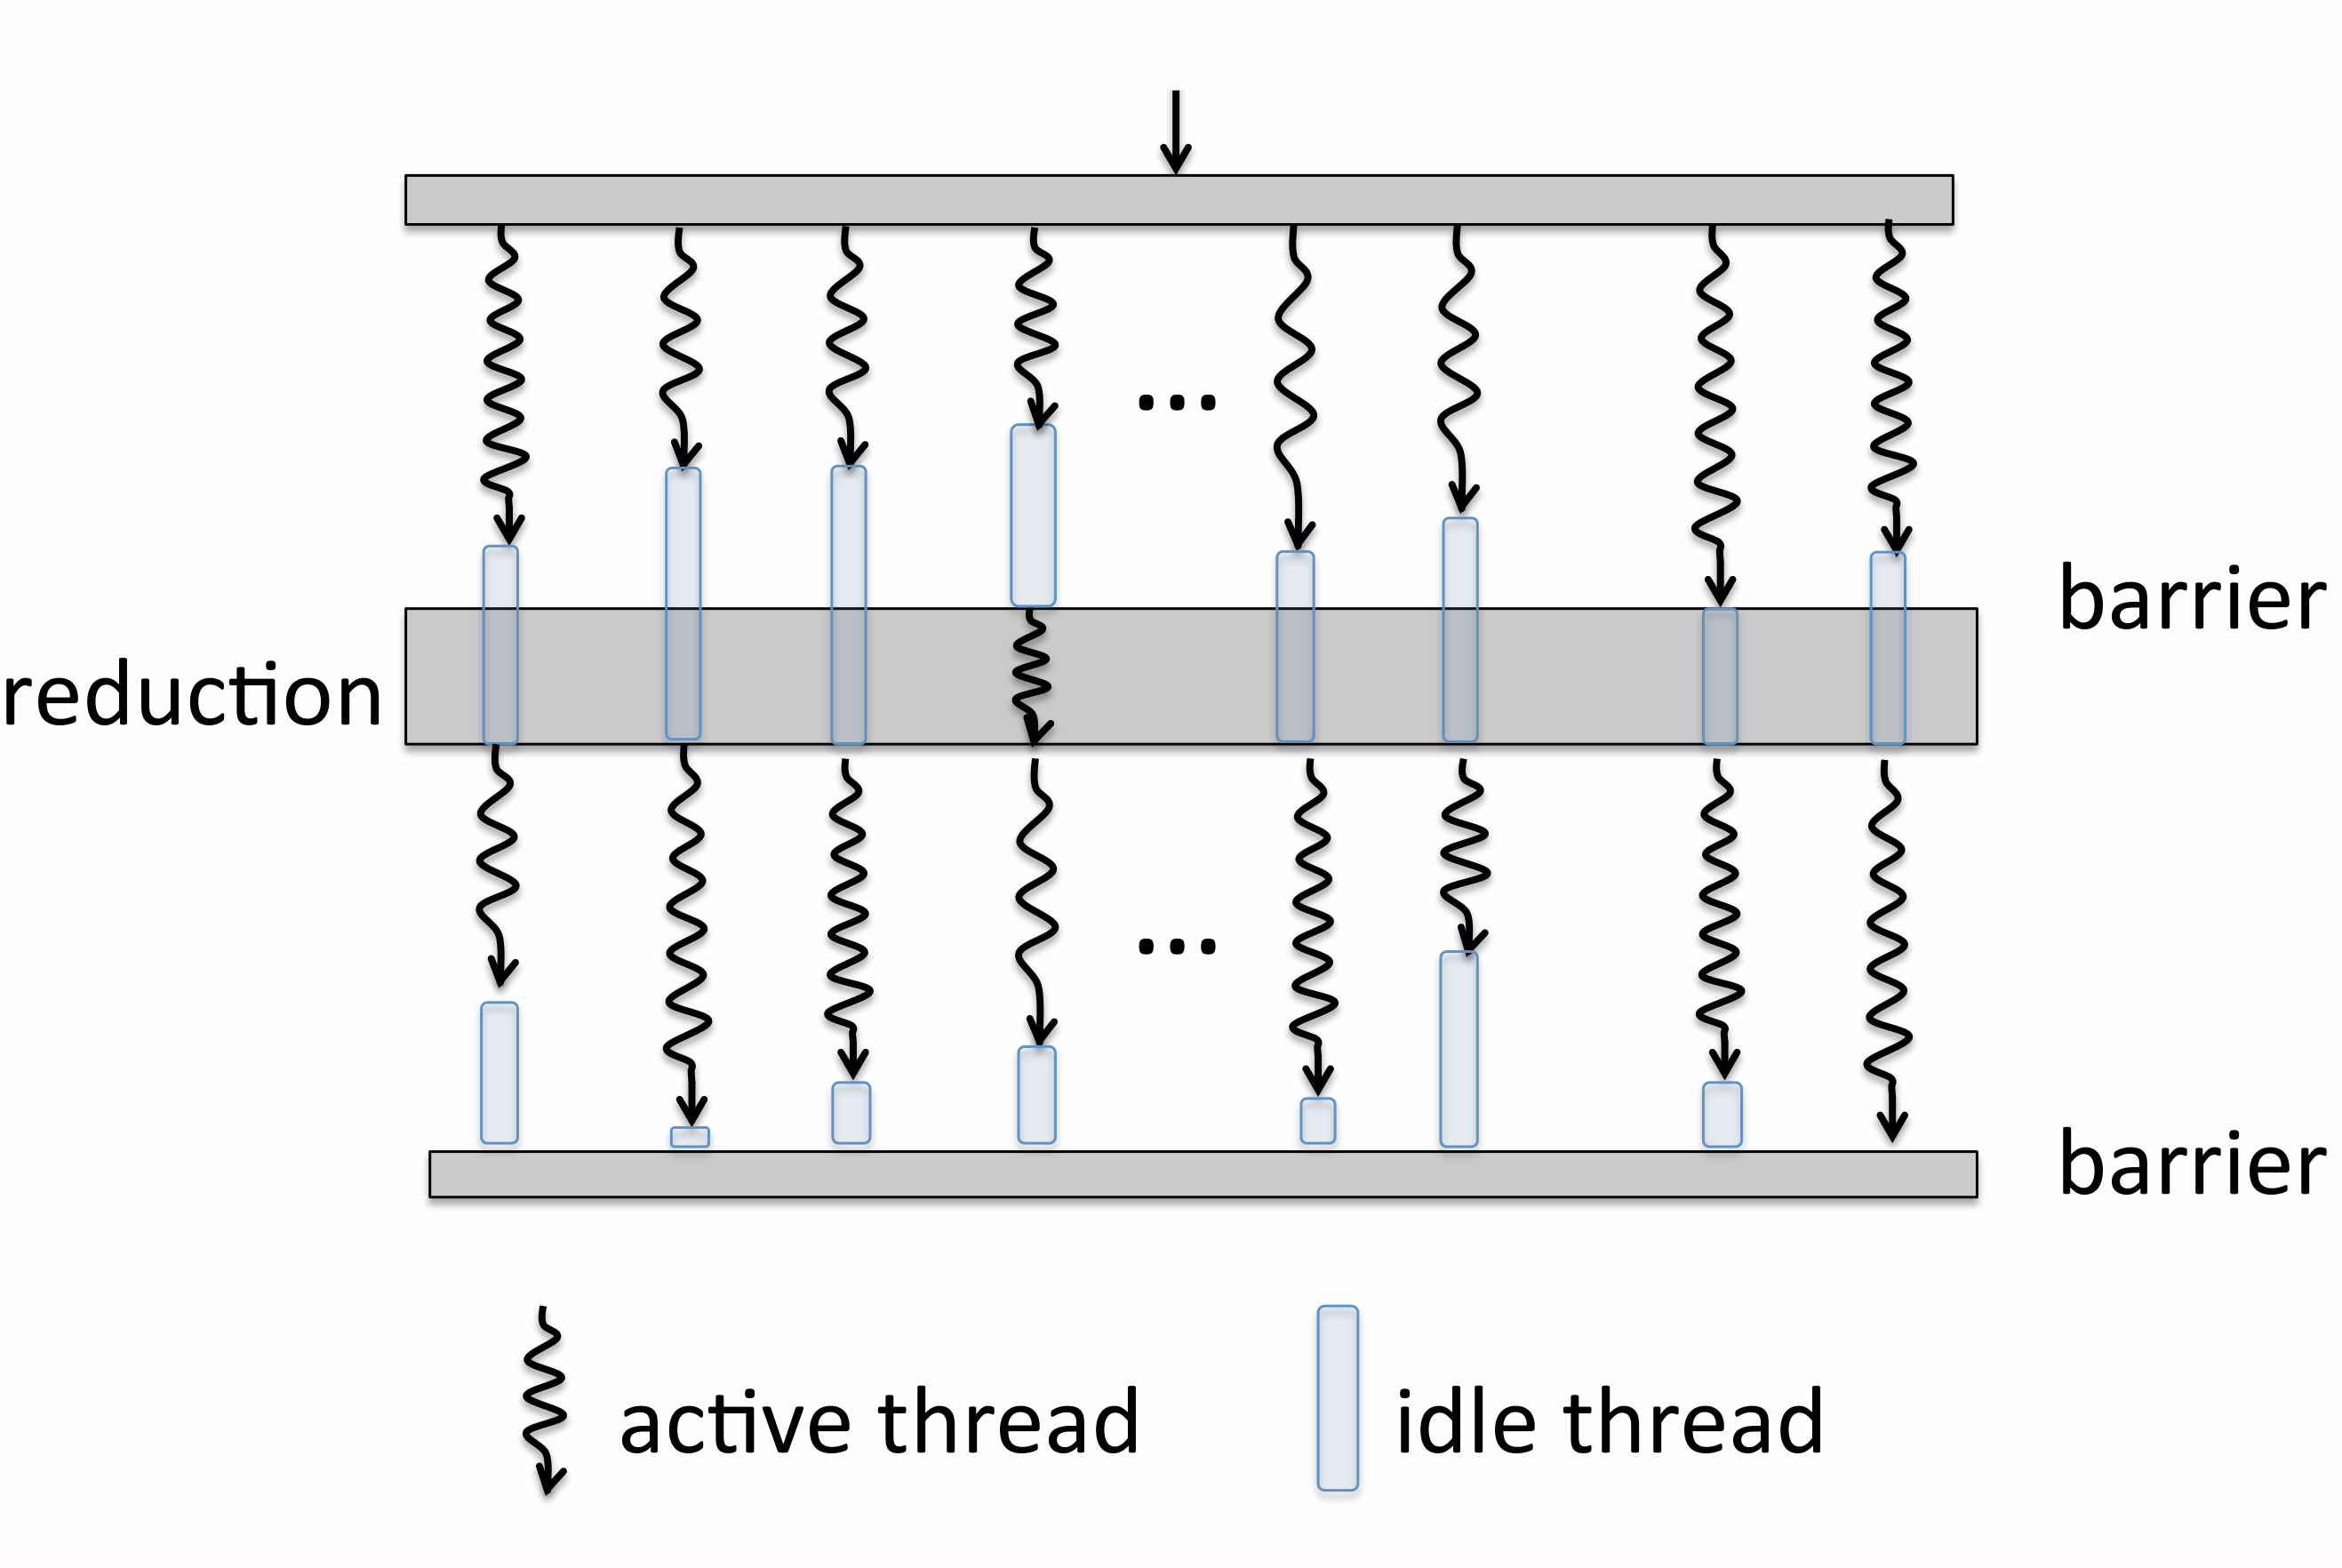
\includegraphics[scale=0.09]{Figures/globalBarriersAndThreadIdleTime.png}
 		\caption{Global barriers and thread idle time\protect\cite{grubel2016dynamic}.
 		This is a representation of how global barriers cause idling on threads with unbalanced workload.
 		We can also see how, during a reduction, just one thread actually operates it while all the others are idle.}
 		\label{fig:globalBarriers}
 	\end{center}
\end{figure}

%eof
